
In Chapter \ref{subsec:controltool} ....






\paragraph{Control system selection}
Based on the arguments for and against certain control system concepts given in section \ref{subsec:controltool} a selection of suitable control system solutions was made. Figure \ref{fig:cgoffset} shows the \gls{cg} offset required along the Z-axis to trim the spacecraft at certain angles of attack for various \gls{cg} locations on the X-axis. 
\begin{figure}[h]
	\centering
	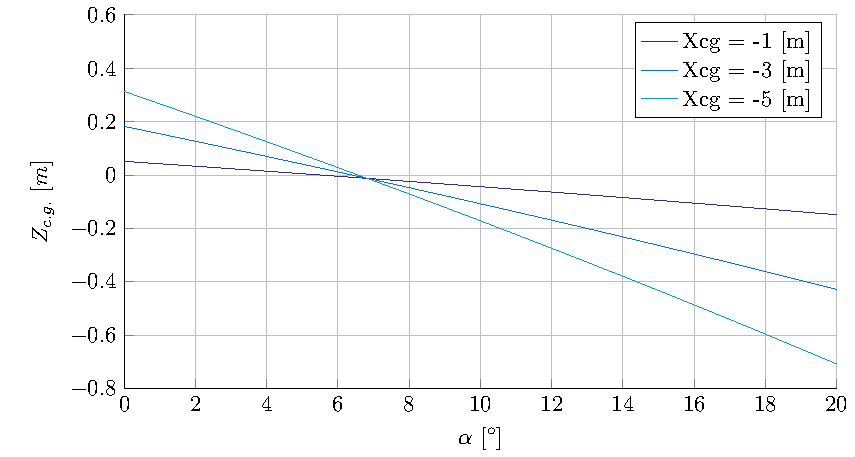
\includegraphics[width=0.95\textwidth]{./Figure/control/moment}
	\caption{1}
	\label{fig:cgoffset}
\end{figure}
From figure \ref{fig:cgoffset} it can be seen that the required \gls{cg} Z-offset grows as the X-offset grows. For an angle of attack change of $2$ degrees corresponding to an X-\gls{cg} located at $-5$ meters a \gls{cg} shift of $0.2$ meters is required. Angle of attack-based trajectory control was found to require trimmed \gls{sym:alpha}-shifts of $5$ degrees that have to be adjusted with a rate of $1$ $deg \cdot s^{-1}$. To pull this off would require the actuation system to produce a \gls{cg} displacement of $0.5$ meters with a required rate of $0.1$ $m \cdot s^{-1}$. This would require excessively heavy actuators that would also have to be able to operate under 3-g loads. Not only has this never been done before in space, the reliability of such a system would be questionable. Based on these arguments a decision was made against active \gls{cg} control.\\
Following the decision to discontinue the consideration of active \gls{cg} control a selection had to be made between the other two control system design options: Body flaps and thrusters. Regarding body flaps some of the same arguments can be made as were used against active \gls{cg} control. Body flaps can require excessively large actuators that are very heavy. In addition to this the dynamic behaviour of the inflatable structure is difficult to compute and can be very unpredictable. Furthermore the use of body flaps on inflatable structures has a very low \acrlong{trl}, which poses an additional development risk. Based on these and other downsides pertaining to aerodynamic control surfaces mentioned in section \ref{subsec:controltool} it was decided to employ thrusters as control system.

\paragraph{Control system results}

The results of the control system can be subdivided into two components. The control system mass and its corresponding accuracy.

Mass estimates are based on the required propellant mass, thruster mass and fuel tank mass. The propellant mass can be subdivided into a further two categories: 